\section{Numerical Tests}

The setup is shown in Fig. \ref{fg:config}, where the heavy (liquid) and light (gas) phases are represented with gray and white colors respectively. The distance $h$ between the cylinder top and the undisturbed free surface is taken as the measure of the cylinder submergence. Uniform inflow velocity with module $U$ is imposed on the inlet. The chosen Froude number based on the diameter of the cylinder $d$ is
\begin{equation}
 Fr = \frac{U}{\sqrt{gd}}
\label{eq:froude}
\end{equation}
where $g$ is the gravity acceleration. Also, the Reynolds number is calculated based on $U$ and $d$ as characteristic velocities and length respectively, being
\begin{equation}
 Re = \frac{U d}{\mu_l}
\label{eq:reynolds}
\end{equation}
with $\mu_l$ the dynamic viscosity of the heavier phase.

\begin{figure}[ht]
  \centering
  %%----primera subfigura----
  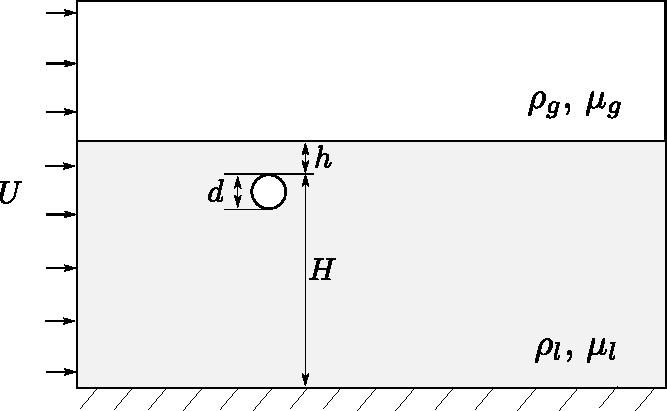
\includegraphics[width=0.9\columnwidth]{images_10thspheric/config.pdf}
  \caption{Case configuration, initial and boundary conditions.}
  \label{fg:config}
\end{figure}

In the reference work of Reichl et.al \cite{Reichl05}, densities and viscosities ratios are established in $\rho_l/\rho_g = \mu_l/\mu_g=100$ in order to avoid convergence problems. PFEM-2 method does not suffer from these drawbacks, allowing more realistic water-air ratios. However, the original ratios are employed to guarantee same simulation conditions. Regarding to boundary conditions, an uniform flow $U$ is imposed at the inlet, leaving free the outlet velocity. The floor of the channel and the cylinder surface are considered no-slip, and atmosphere condition is set at the top of the geometry.

Flow conditions are inspirated in the work of Bouscasse \cite{Bouscasse14} which investigates the flow behavior employing a range of Froude numbers for a fixed submergence ($h/d=0.55$ ratio) and a fixed Reynolds number of $Re=180$. The mentioned reference uses SPH as numerical method allowing to treat larger fragmentation of the free surface, compared to FLUENT-VOF technique used by Reichl and colleagues. The PFEM-2 method employed in the current work, since its particle nature, is also able to treat large deformations and breakups.

Figure \ref{fg:vort_Re180} presents the influence of the Froude number in the flow characteristics, represented by the dimensionless vorticity. Simulating with the lower Froude $Fr=0.3$, the free-surface acts as a no-slip wall because it hardly gets deformed and the vortex production presents similar behavior to one-phase tests \cite{PRICE2002175}. As the Froude number increases from 0.3, the physics changes dramatically. Although the free-surface remains almost flat, the vortex production is completely blocked. Also, a recirculation area appears just behind the cylinder and close to the free-surface, the positive vorticity generated at the free surface by the spilling breaker builds up a large positive meta-vortex behind the cylinder which is then advected downstream. Reaching intermediate-high Froude numbers (1.2 and 1.6) structures developed are not periodic, while as the vortex production remains blocked due to the continuous breakups ocurring at free-surface. The analysis from 0.3 to 1.6 is in agreement with the work of Bouscasse et. al \cite{Bouscasse14}.

When the analysis for $Fr=2.0$ is done, differences between the flow characteristics of the mentioned reference and this current work are found. Bouscasse shows that at this Froude number the vortex production is recovered while our results find instabilities but not shedding. In order to present a regime where the like von karman street appear, a case with $Fr=3.5$ was also run finding vortex shedding behind the cylinder and large distortions of the free-surface but without the characteristic chaos of the intermediate Froude numbers.


\begin{figure}[htbp]
  \begin{center}
    \subfloat[$Fr=0.3$]{
	  \label{fg:vort_a}
	  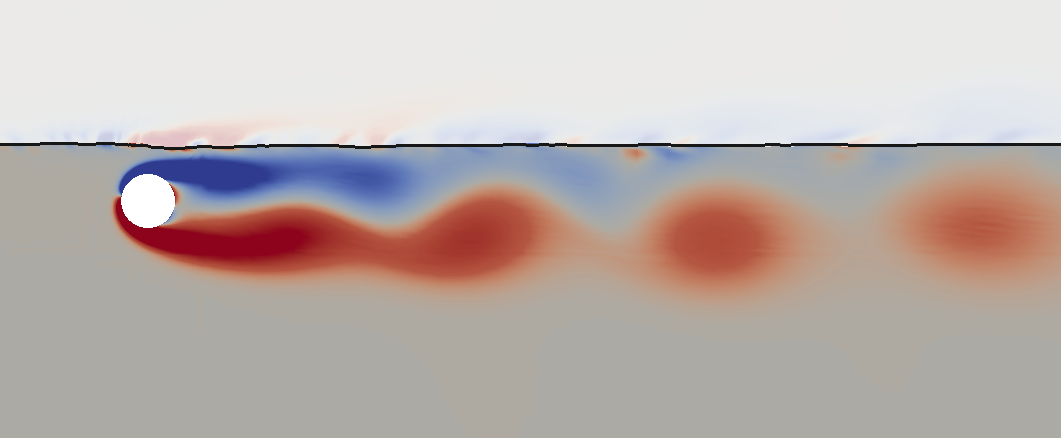
\includegraphics[width=.9\columnwidth]{images_10thspheric/Fr_0_3_Re_180_h_0_55_vorticity.png}
    } \\
\subfloat[$Fr=0.6$]{
	  \label{fg:vort_b}
	  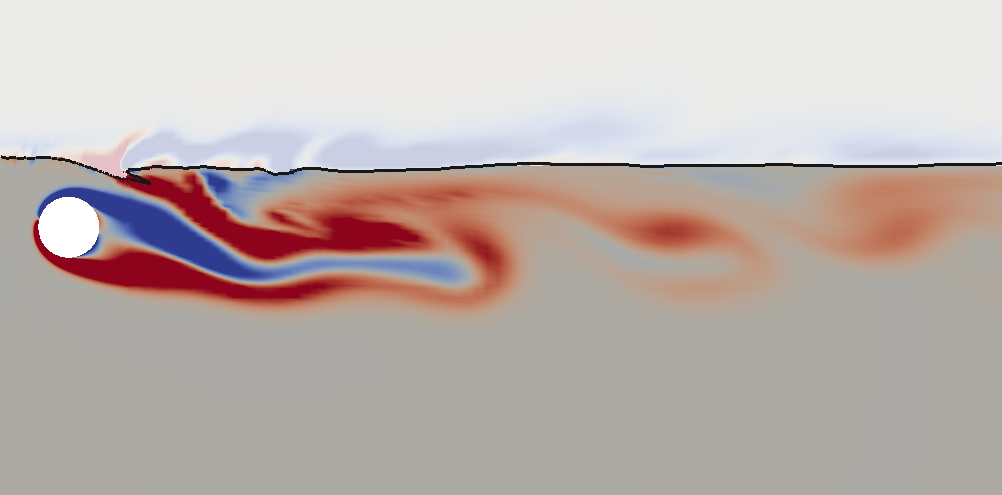
\includegraphics[width=.9\columnwidth]{images_10thspheric/Fr_0_6_Re_180_h_0_55_vorticity.png}
    } \\
% \subfloat[$Fr=0.8$]{
% 	  \label{fg:vort_c}
% 	  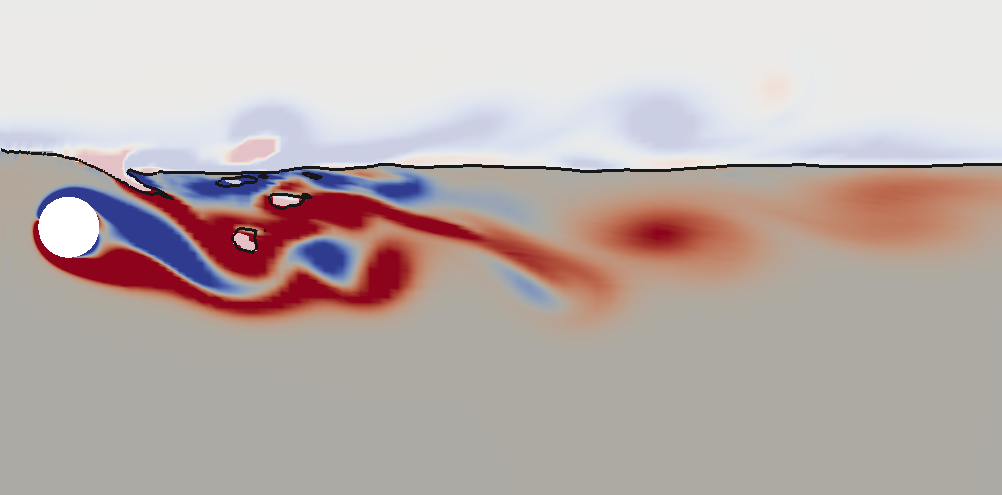
\includegraphics[width=.9\columnwidth]{images_10thspheric/Fr_0_8_Re_180_h_0_55_vorticity.png}
%     } \\
\subfloat[$Fr=1.2$]{
	  \label{fg:vort_d}
	  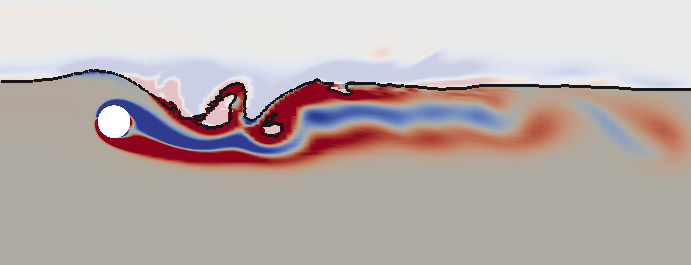
\includegraphics[width=.9\columnwidth]{images_10thspheric/Fr_1_2_Re_180_h_0_55_vorticity.png}
    } \\
\subfloat[$Fr=1.6$]{
	  \label{fg:vort_e}
	  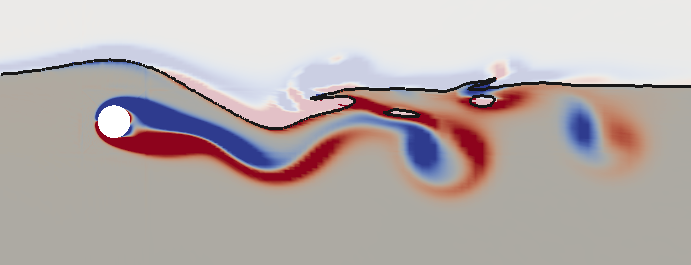
\includegraphics[width=.9\columnwidth]{images_10thspheric/Fr_1_6_Re_180_h_0_55_vorticity.png}
    } \\ 
\subfloat[$Fr=2.0$]{
	  \label{fg:vort_f}
	  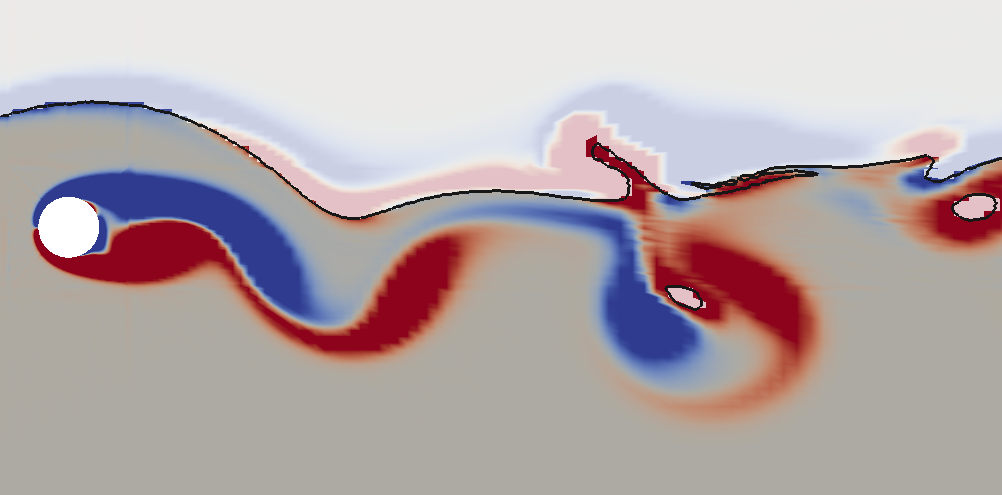
\includegraphics[width=.9\columnwidth]{images_10thspheric/Fr_2_0_Re_180_h_0_55_vorticity.png}
    } \\ 
\subfloat[$Fr=3.5$]{
	  \label{fg:vort_g}
	  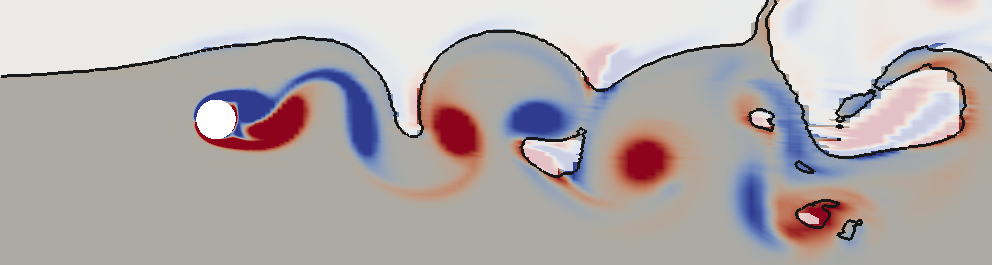
\includegraphics[width=.9\columnwidth]{images_10thspheric/Fr_3_5_Re_180_h_0_55_vorticity.png}
    } \\ 
  \end{center}
  \caption{\label{fg:vort_Re180} Influence of Froude number on dimensionless vorticity $\hat\omega = curl(\vv) \sqrt{d/g}$ (scales from -3 (blue) to 3 (red)) with $h/d = 0.55$ and $Re=180$. Captures at $t^*=80$.
}
\end{figure}


A summary of computed forces can be seen in Fig. \ref{fg:CdCl}. The drag coefficient slightly diminishes as Froude number increases. A maximum lift (in absolute value) is found for $Fr = 0.8$, and then a gentle monotonic reduction for the largest Froude number cases occurs. Good agreement with the reference work can be observed.

\begin{figure}[ht]
  \centering
  %%----primera subfigura----
  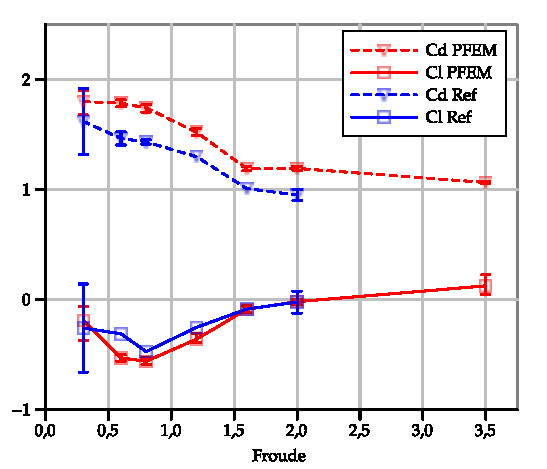
\includegraphics[width=0.95\columnwidth]{images_10thspheric/CdCl_Re180_hd_0_55.pdf}
  \caption{Drag and Lift coefficients calculated with PFEM-2 compared with the reference work of Bouscasse \cite{Bouscasse14}. $Re=180$.} %, $t^*=tU/d$. }
  \label{fg:CdCl}
\end{figure}